\documentclass{standalone}
\usepackage{tikz}
\usetikzlibrary{patterns}
\usetikzlibrary{positioning}
\usetikzlibrary{patterns, positioning}
\usetikzlibrary{shapes.misc}
\usepackage[outline]{contour}
\contourlength{1.5pt} 
\usepackage[sfdefault]{ClearSans}

\begin{document}
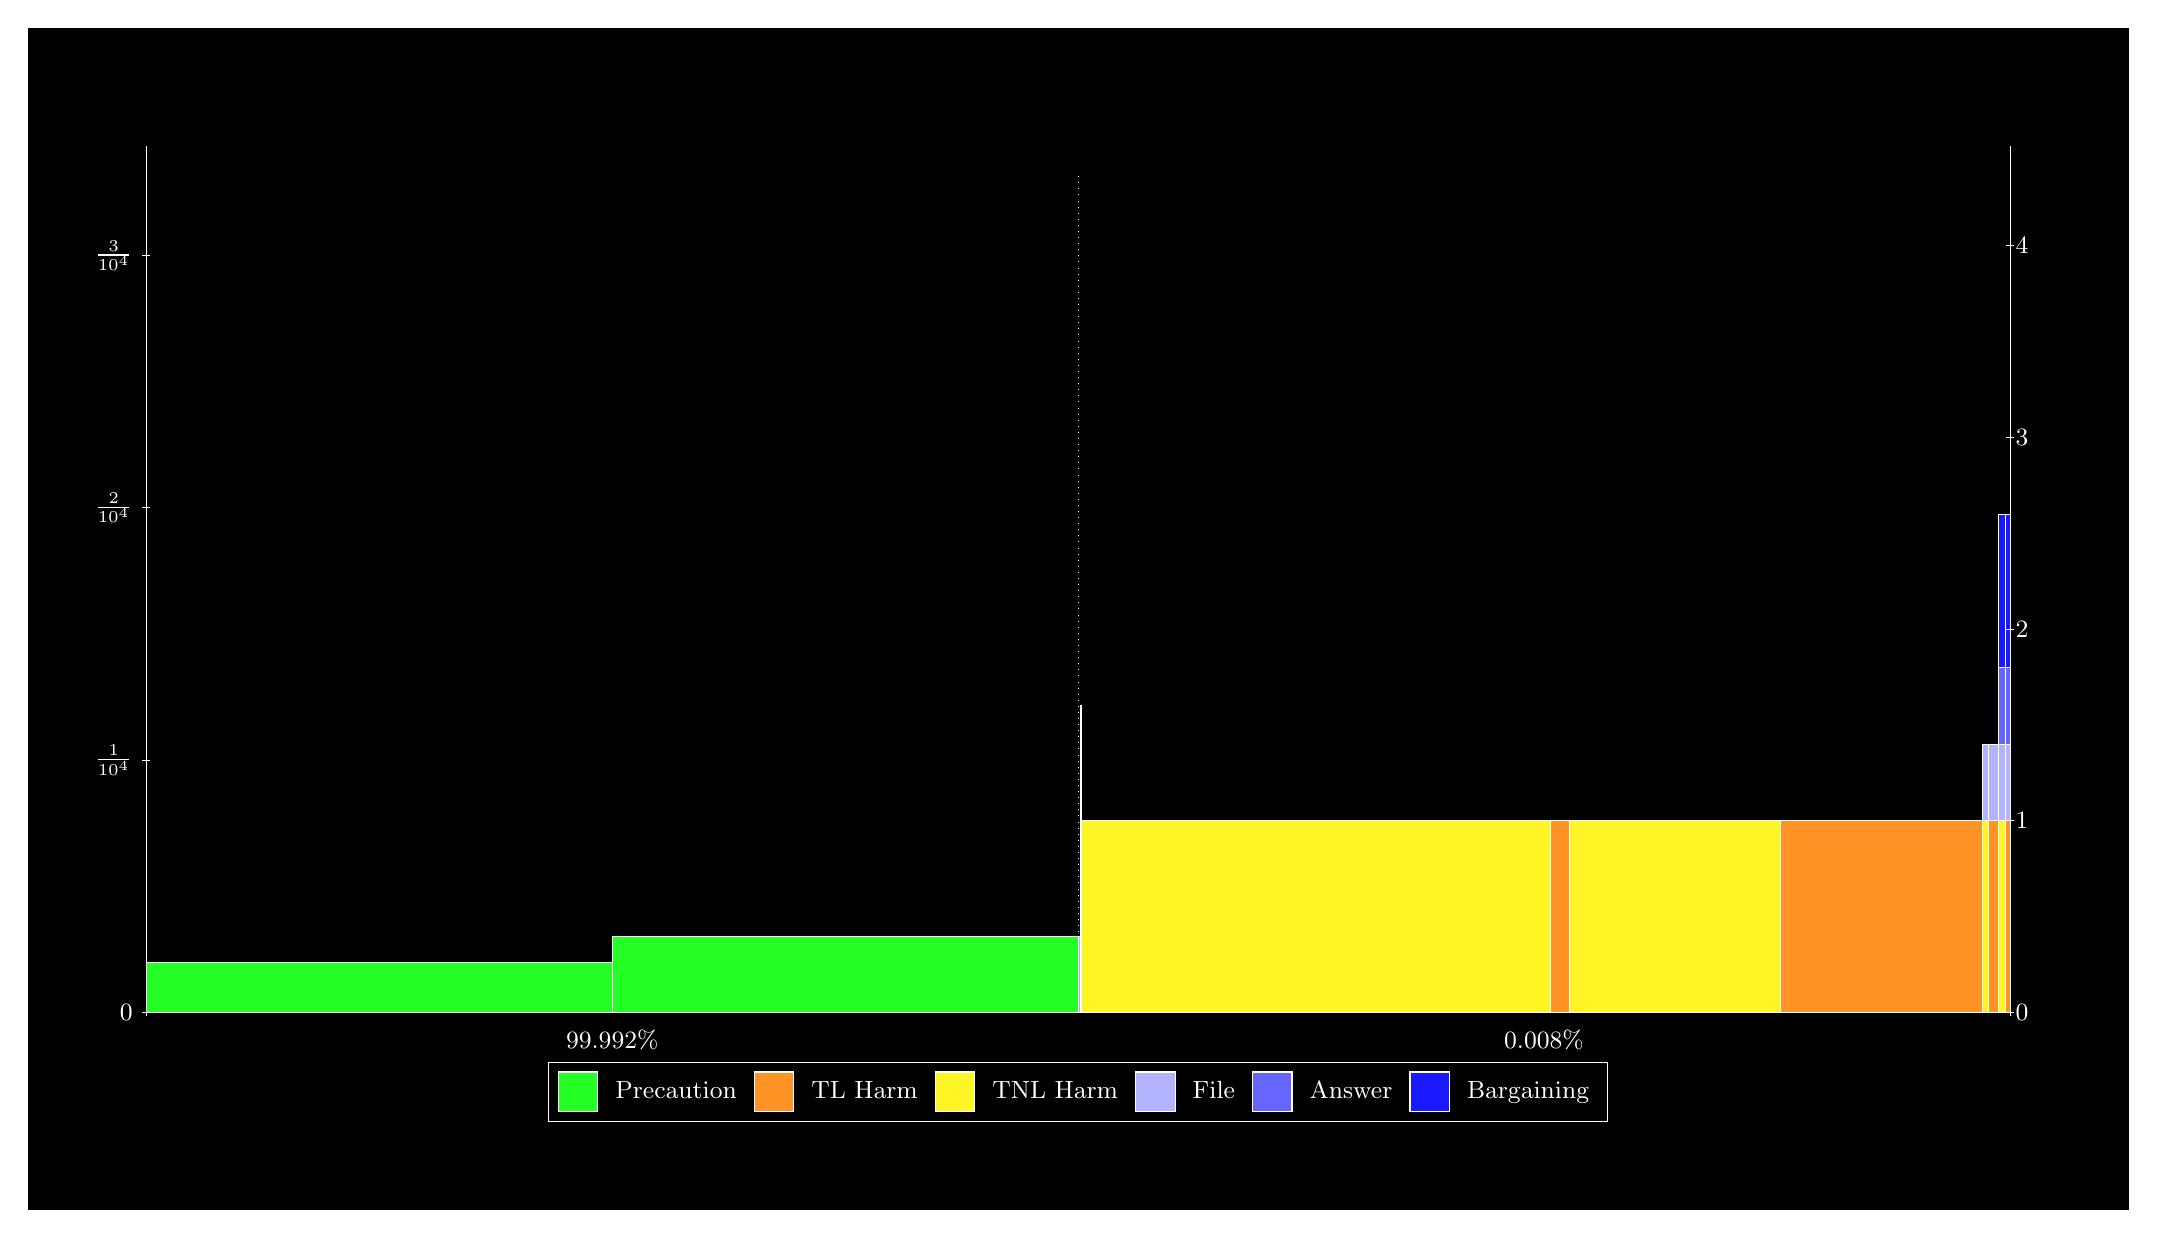
\begin{tikzpicture}
\draw[fill=black] (0,0) rectangle (26.667,15);
\draw[fill=green!85,draw=white,very thin] (1.5,2.5) rectangle (7.4166,3.141);
\draw[fill=green!85,draw=white,very thin] (7.4166,2.5) rectangle (13.333,3.4616);
\draw[fill=green!85,draw=white,very thin] (13.333,2.5) rectangle (13.36,2.5);
\draw[fill=blue!30,draw=white,very thin] (13.333,2.5) rectangle (13.36,3.474);
\draw[fill=green!85,draw=white,very thin] (13.36,2.5) rectangle (13.378,2.5);
\draw[fill=blue!30,draw=white,very thin] (13.36,2.5) rectangle (13.378,3.474);
\draw[fill=blue!60,draw=white,very thin] (13.36,3.474) rectangle (13.378,4.4479);
\draw[fill=blue!90,draw=white,very thin] (13.36,4.4479) rectangle (13.378,6.3958);
\draw[fill=green!85,draw=white,very thin] (13.378,2.5) rectangle (19.334,2.5);
\draw[fill=yellow!85,draw=white,very thin] (13.378,2.5) rectangle (19.334,4.9349);
\draw[fill=green!85,draw=white,very thin] (19.334,2.5) rectangle (19.577,2.5);
\draw[fill=orange!85,draw=white,very thin] (19.334,2.5) rectangle (19.577,4.9349);
\draw[fill=green!85,draw=white,very thin] (19.577,2.5) rectangle (22.255,2.5001);
\draw[fill=yellow!85,draw=white,very thin] (19.577,2.5001) rectangle (22.255,4.9349);
\draw[fill=green!85,draw=white,very thin] (22.255,2.5) rectangle (24.815,2.5001);
\draw[fill=orange!85,draw=white,very thin] (22.255,2.5001) rectangle (24.815,4.9349);
\draw[fill=green!85,draw=white,very thin] (24.815,2.5) rectangle (24.888,2.5);
\draw[fill=yellow!85,draw=white,very thin] (24.815,2.5) rectangle (24.888,4.9349);
\draw[fill=blue!30,draw=white,very thin] (24.815,4.9349) rectangle (24.888,5.9089);
\draw[fill=green!85,draw=white,very thin] (24.888,2.5) rectangle (25.02,2.5);
\draw[fill=orange!85,draw=white,very thin] (24.888,2.5) rectangle (25.02,4.9349);
\draw[fill=blue!30,draw=white,very thin] (24.888,4.9349) rectangle (25.02,5.9089);
\draw[fill=green!85,draw=white,very thin] (25.02,2.5) rectangle (25.114,2.5);
\draw[fill=yellow!85,draw=white,very thin] (25.02,2.5) rectangle (25.114,4.9349);
\draw[fill=blue!30,draw=white,very thin] (25.02,4.9349) rectangle (25.114,5.9089);
\draw[fill=blue!60,draw=white,very thin] (25.02,5.9089) rectangle (25.114,6.8828);
\draw[fill=blue!90,draw=white,very thin] (25.02,6.8828) rectangle (25.114,8.8307);
\draw[fill=green!85,draw=white,very thin] (25.114,2.5) rectangle (25.167,2.5);
\draw[fill=orange!85,draw=white,very thin] (25.114,2.5) rectangle (25.167,4.9349);
\draw[fill=blue!30,draw=white,very thin] (25.114,4.9349) rectangle (25.167,5.9089);
\draw[fill=blue!60,draw=white,very thin] (25.114,5.9089) rectangle (25.167,6.8828);
\draw[fill=blue!90,draw=white,very thin] (25.114,6.8828) rectangle (25.167,8.8307);
\draw[white,very thin] (1.5,2.5) -- (1.5,13.5);
\draw[white,very thin] (1.45,2.5) -- (1.55,2.5);
\node[font=\small,text=white, anchor=east] at (1.45, 2.5) {0};
\draw[white,very thin] (1.45,5.7052) -- (1.55,5.7052);
\node[font=\small,text=white, anchor=east] at (1.45, 5.7052) {$\frac{1}{10^{4}}$};
\draw[white,very thin] (1.45,8.9104) -- (1.55,8.9104);
\node[font=\small,text=white, anchor=east] at (1.45, 8.9104) {$\frac{2}{10^{4}}$};
\draw[white,very thin] (1.45,12.116) -- (1.55,12.116);
\node[font=\small,text=white, anchor=east] at (1.45, 12.116) {$\frac{3}{10^{4}}$};

\draw[white,dotted,very thin] (13.333,2.83) -- (13.333,13.17);
\draw[white,very thin] (25.167,2.5) -- (25.167,13.5);
\draw[white,very thin] (25.117,2.5) -- (25.217,2.5);
\node[font=\small,text=white, anchor=west] at (25.117, 2.5) {0};
\draw[white,very thin] (25.117,4.9349) -- (25.217,4.9349);
\node[font=\small,text=white, anchor=west] at (25.117, 4.9349) {1};
\draw[white,very thin] (25.117,7.3697) -- (25.217,7.3697);
\node[font=\small,text=white, anchor=west] at (25.117, 7.3697) {2};
\draw[white,very thin] (25.117,9.8046) -- (25.217,9.8046);
\node[font=\small,text=white, anchor=west] at (25.117, 9.8046) {3};
\draw[white,very thin] (25.117,12.239) -- (25.217,12.239);
\node[font=\small,text=white, anchor=west] at (25.117, 12.239) {4};

\draw[white,very thin] (1.5,2.5) -- (25.167,2.5);
\draw[white,very thin] (1.5,2.45) -- (1.5,2.55);
\node[font=\small,text=white, anchor=north] at (1.5, 2.45) {};
\draw[white,very thin] (25.167,2.45) -- (25.167,2.55);
\node[font=\small,text=white, anchor=north] at (25.167, 2.45) {};

\node[font=\small,text=white,anchor=south] at (7.4167, 1.9) {99.992\%};
\node[font=\small,text=white,anchor=south] at (19.25, 1.9) {0.008\%};
\draw (13.3333,2.5) node (B) {};
\begin{scope}[align=center]
\matrix[scale=0.5,draw=white,below=0.5cm of B,nodes={draw},column sep=0.1cm]{
\node[rectangle,draw,minimum width=0.5cm,minimum height=0.5cm,fill=green!85]{}; & \node[draw=none,font=\small,text=white]{Precaution}; &
\node[rectangle,draw,minimum width=0.5cm,minimum height=0.5cm,fill=orange!85]{}; & \node[draw=none,font=\small,text=white]{TL Harm}; &
\node[rectangle,draw,minimum width=0.5cm,minimum height=0.5cm,fill=yellow!85]{}; & \node[draw=none,font=\small,text=white]{TNL Harm}; &
\node[rectangle,draw,minimum width=0.5cm,minimum height=0.5cm,fill=blue!30]{}; & \node[draw=none,font=\small,text=white]{File}; &
\node[rectangle,draw,minimum width=0.5cm,minimum height=0.5cm,fill=blue!60]{}; & \node[draw=none,font=\small,text=white]{Answer}; &
\node[rectangle,draw,minimum width=0.5cm,minimum height=0.5cm,fill=blue!90]{}; & \node[draw=none,font=\small,text=white]{Bargaining}; \\\\
};\end{scope}

\end{tikzpicture}
\end{document}